\documentclass[pdf,aspectratio=169]{beamer}
\usepackage[]{hyperref,graphicx,siunitx,lmodern,booktabs,tikz,tensor}
\usepackage{pgfplots,pgfplotstable}
\usepackage{pdfpc-commands}

%\usepackage{pgfpages}
%\pgfpagesuselayout{4 on 1}[letterpaper, border shrink=5mm, landscape]
\usepackage[mode=buildnew]{standalone}
\mode<presentation>{\usetheme{Astro}}

\graphicspath{ {../Images/} }

\sisetup{per-mode=symbol}
\usetikzlibrary{calc,intersections, decorations.pathmorphing,shadings,positioning}
%\tikzstyle{proton}=[circle, minimum size = 7mm, ball color=red, black,transform shape]
%\tikzstyle{neutron}=[circle, minimum size=7mm, ball color=gray, black, transform shape]
%\tikzstyle{gammaray}=[ultra thick, -latex, decorate, decoration={snake, post length=3mm}]


%preamble
\title{Back to the Beginning}
\date{December 5, 2018}
\author{Jed Rembold}

\begin{document}
\renewcommand*{\theenumi}{\Alph{enumi}}

\begin{frame}{Announcements}
  \begin{itemize}
	  \item Last Webwork (ever!) due on Friday!
	  \item On Friday:
		  \begin{itemize}
		  	\item Aliens!
			\item Evaluations! (of me)!
			\item Please show up!
		  \end{itemize}
	\item Final next Wednesday!
	  \begin{itemize}
		\item 8am here!
		\item Study materials posted!
		\item Bring your calculator or email me if you need to borrow one
		\item I'll be around at least all afternoon Monday and Tuesday for questions or Campuswire
	  \end{itemize}
	  \item I've opened up all old homeworks for the max 75\% credit until the date of the final. If you missed one or never completed one, now is your chance!
	\item Polling: \url{rembold-class.ddns.net}
  \end{itemize}
\end{frame}

\begin{frame}{Review Question}
	What is the current best description of dark energy?
	\begin{enumerate}
		\item Energy associated with the movement of dark matter
		\item \alert<2>{Energy that drives the increasing expansion rate of the universe}
		\item Energy released with dark matter and normal matter interact
		\item Energy associated with the redshifted movement of distant galaxies
	\end{enumerate}
\end{frame}


%\begin{frame}{The Galactic Timeline}
  %\begin{center}
	%\begin{tikzpicture}
	  %\begin{axis}[
		  %width=10cm,
		  %height=7cm,
		  %xlabel= Billions of Years,
		  %ylabel= Relative Size of Universe,
		  %ymin=0.1, ymax=4,
		  %xmax=30,
		%]
		%\addplot[mark=none, red, ultra thick] table[x index=0, y index=1] {../Data/3and7.csv};
		%\addplot[mark=none, cyan, ultra thick] table[x index=0, y index=1] {../Data/3and0.csv};
		%\addplot[mark=none, green, ultra thick] table[x index=0, y index=1] {../Data/1and0.csv};
		%\addplot[mark=none, orange, ultra thick,smooth] table[x index=0, y index=1] {../Data/5and0.csv};
		%\node (1) at (axis cs: -8,3.5) {$\Omega_m \qquad \Omega_v$};
		%\node[below =0.5mm of 1,red] (2) {0.3\qquad0.7};
		%\node[below =0.5mm of 2,cyan] (3) {0.3\qquad0.0};
		%\node[below =0.5mm of 3,green] (4) {1.0\qquad0.0};
		%\node[below =0.5mm of 4,orange] (4) {5.0\qquad0.0};
	  %\end{axis}
	%\end{tikzpicture}
  %\end{center}
%\end{frame}

\begin{frame}{Flat and Expanding}
  \begin{itemize}
	\item Note that the sum of the two density factors now gives a value of 1
	  \begin{itemize}
		\item Supporting the findings that the universe seems to be flat!
	  \end{itemize}
	\item Dark energy provides the extra 70\% of the mass/energy of the universe
	\item Results in an age of the universe very similar to the 14 billion years estimated from a constant expansion rate
	\item So, as far as we know, at the moment we think that our universe is:
	  \begin{itemize}
		\item Flat
		\item Expanding increasingly quickly
		\item About 14 billion years old
		\item Infinite or Finite is not well determined yet
	  \end{itemize}
  \end{itemize}
\end{frame}

\begin{frame}{Taking it Back}
  \begin{columns}
	\column{.5\textwidth}
	\begin{itemize}
	  \item Long ago the universe was denser
	  \item And hotter
	  \item Can we look back far enough to ``see'' this ``era''?
	\end{itemize}
	\column{.5\textwidth}
	\begin{center}
	  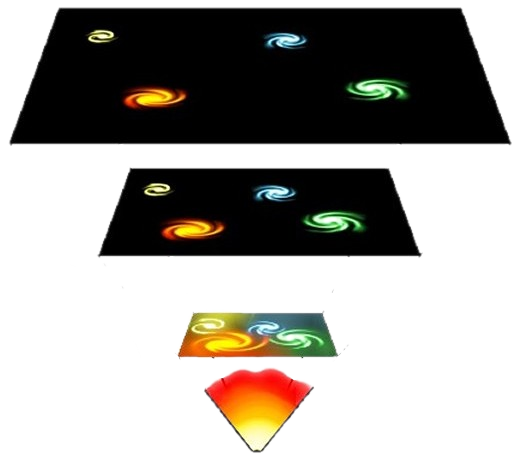
\includegraphics[width=\textwidth]{ch18_expanding.png}
	\end{center}
  \end{columns}
\end{frame}

\begin{frame}{Physics In Reverse}
  \begin{itemize}
	\item Moving backwards, and using what we know about stars, nuclear physics, and everything else, the history of the universe looks something like below:
  \end{itemize}
  \begin{center}
	  \begin{tikzpicture}
		  \node[inner sep=0pt, outer sep=0pt](pic1) at (0,0) {\includegraphics[width=.495\textwidth]{ch18_universehistory1.jpg}};
		  \node[inner sep=0pt, outer sep=0pt,anchor=west] at (pic1.east) {\includegraphics[width=.495\textwidth]{ch18_universehistory2.jpg}};
	  \end{tikzpicture}
  \end{center}
\end{frame}

\begin{frame}{How far back COULD we see?}
  \begin{itemize}
	\item Assuming perfect and huge telescopes, how far back could we see?
	\item Early universe very very hot
	  \begin{itemize}
		\item Hot enough for fusion
		\item Hot enough that particles are charged
		\item Fusion releases radiation, that interacts with particles
		\item Light gets scattered $\Rightarrow$ opaque
	  \end{itemize}
	\item Once it cooled enough for non-ionized atoms to form, radiation no longer interacts
	  \begin{itemize}
		\item Can travel long distances
		\item Transparent
	  \end{itemize}
	\item Called ``Recombination''
  \end{itemize}
\end{frame}

%\begin{frame}{Review Question}
  %Comparing models of the shape and structure of the universe to observed Type I supernova currently predict that the universe has:
  %\begin{enumerate}
	%\item flat curvature and about 30\% dark energy
	%\item negative curvature and about 30\% dark energy
	%\item positive curvature and 5\% dark energy
	%\item flat curvature and is about 70\% dark energy
  %\end{enumerate}
%\end{frame}

\begin{frame}{Recombination}
  \begin{columns}
	\column{.5\textwidth}
	\begin{itemize}
	  \item Recombination is when the universe cooled to the point that atoms could become un-ionized and group together
	  \item Allowed photons to pass through unhindered
	  \item Universe became transparent (mostly)
	  \item Models predict recombination should have happened several hundred thousand years after the Big Bang
	\end{itemize}
	\column{.5\textwidth}
	\begin{center}
	  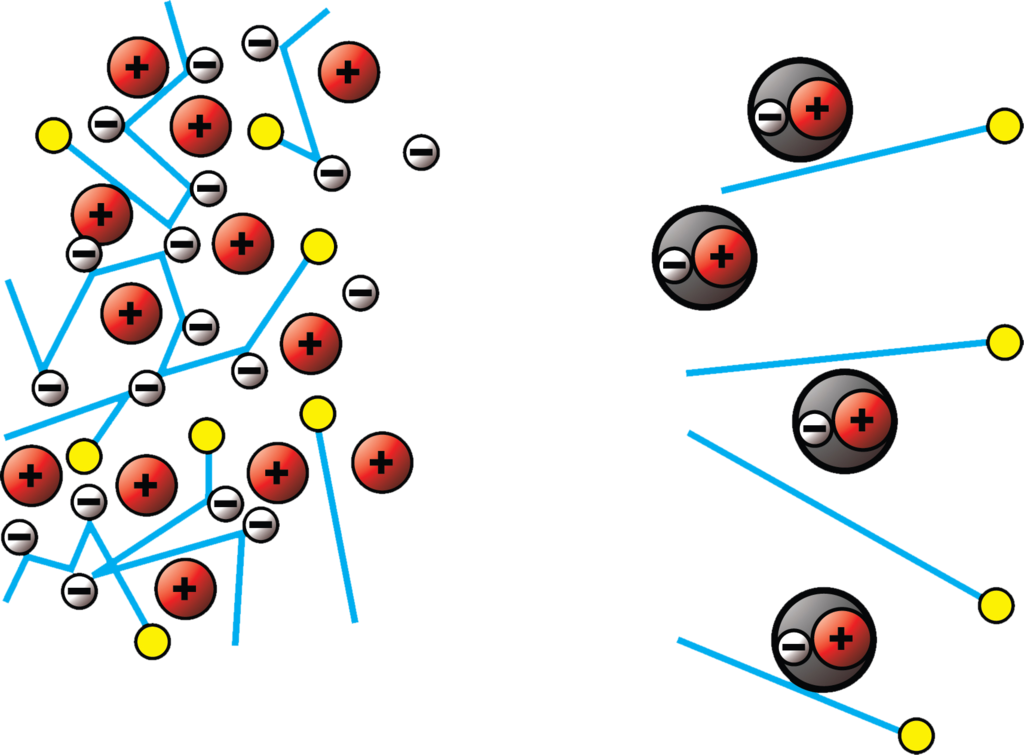
\includegraphics[width=\textwidth]{ch18_recombination.png}
	\end{center}
  \end{columns}
\end{frame}

\begin{frame}{Background Radiation}
  \begin{columns}
	\column{.5\textwidth}
	\begin{center}
	  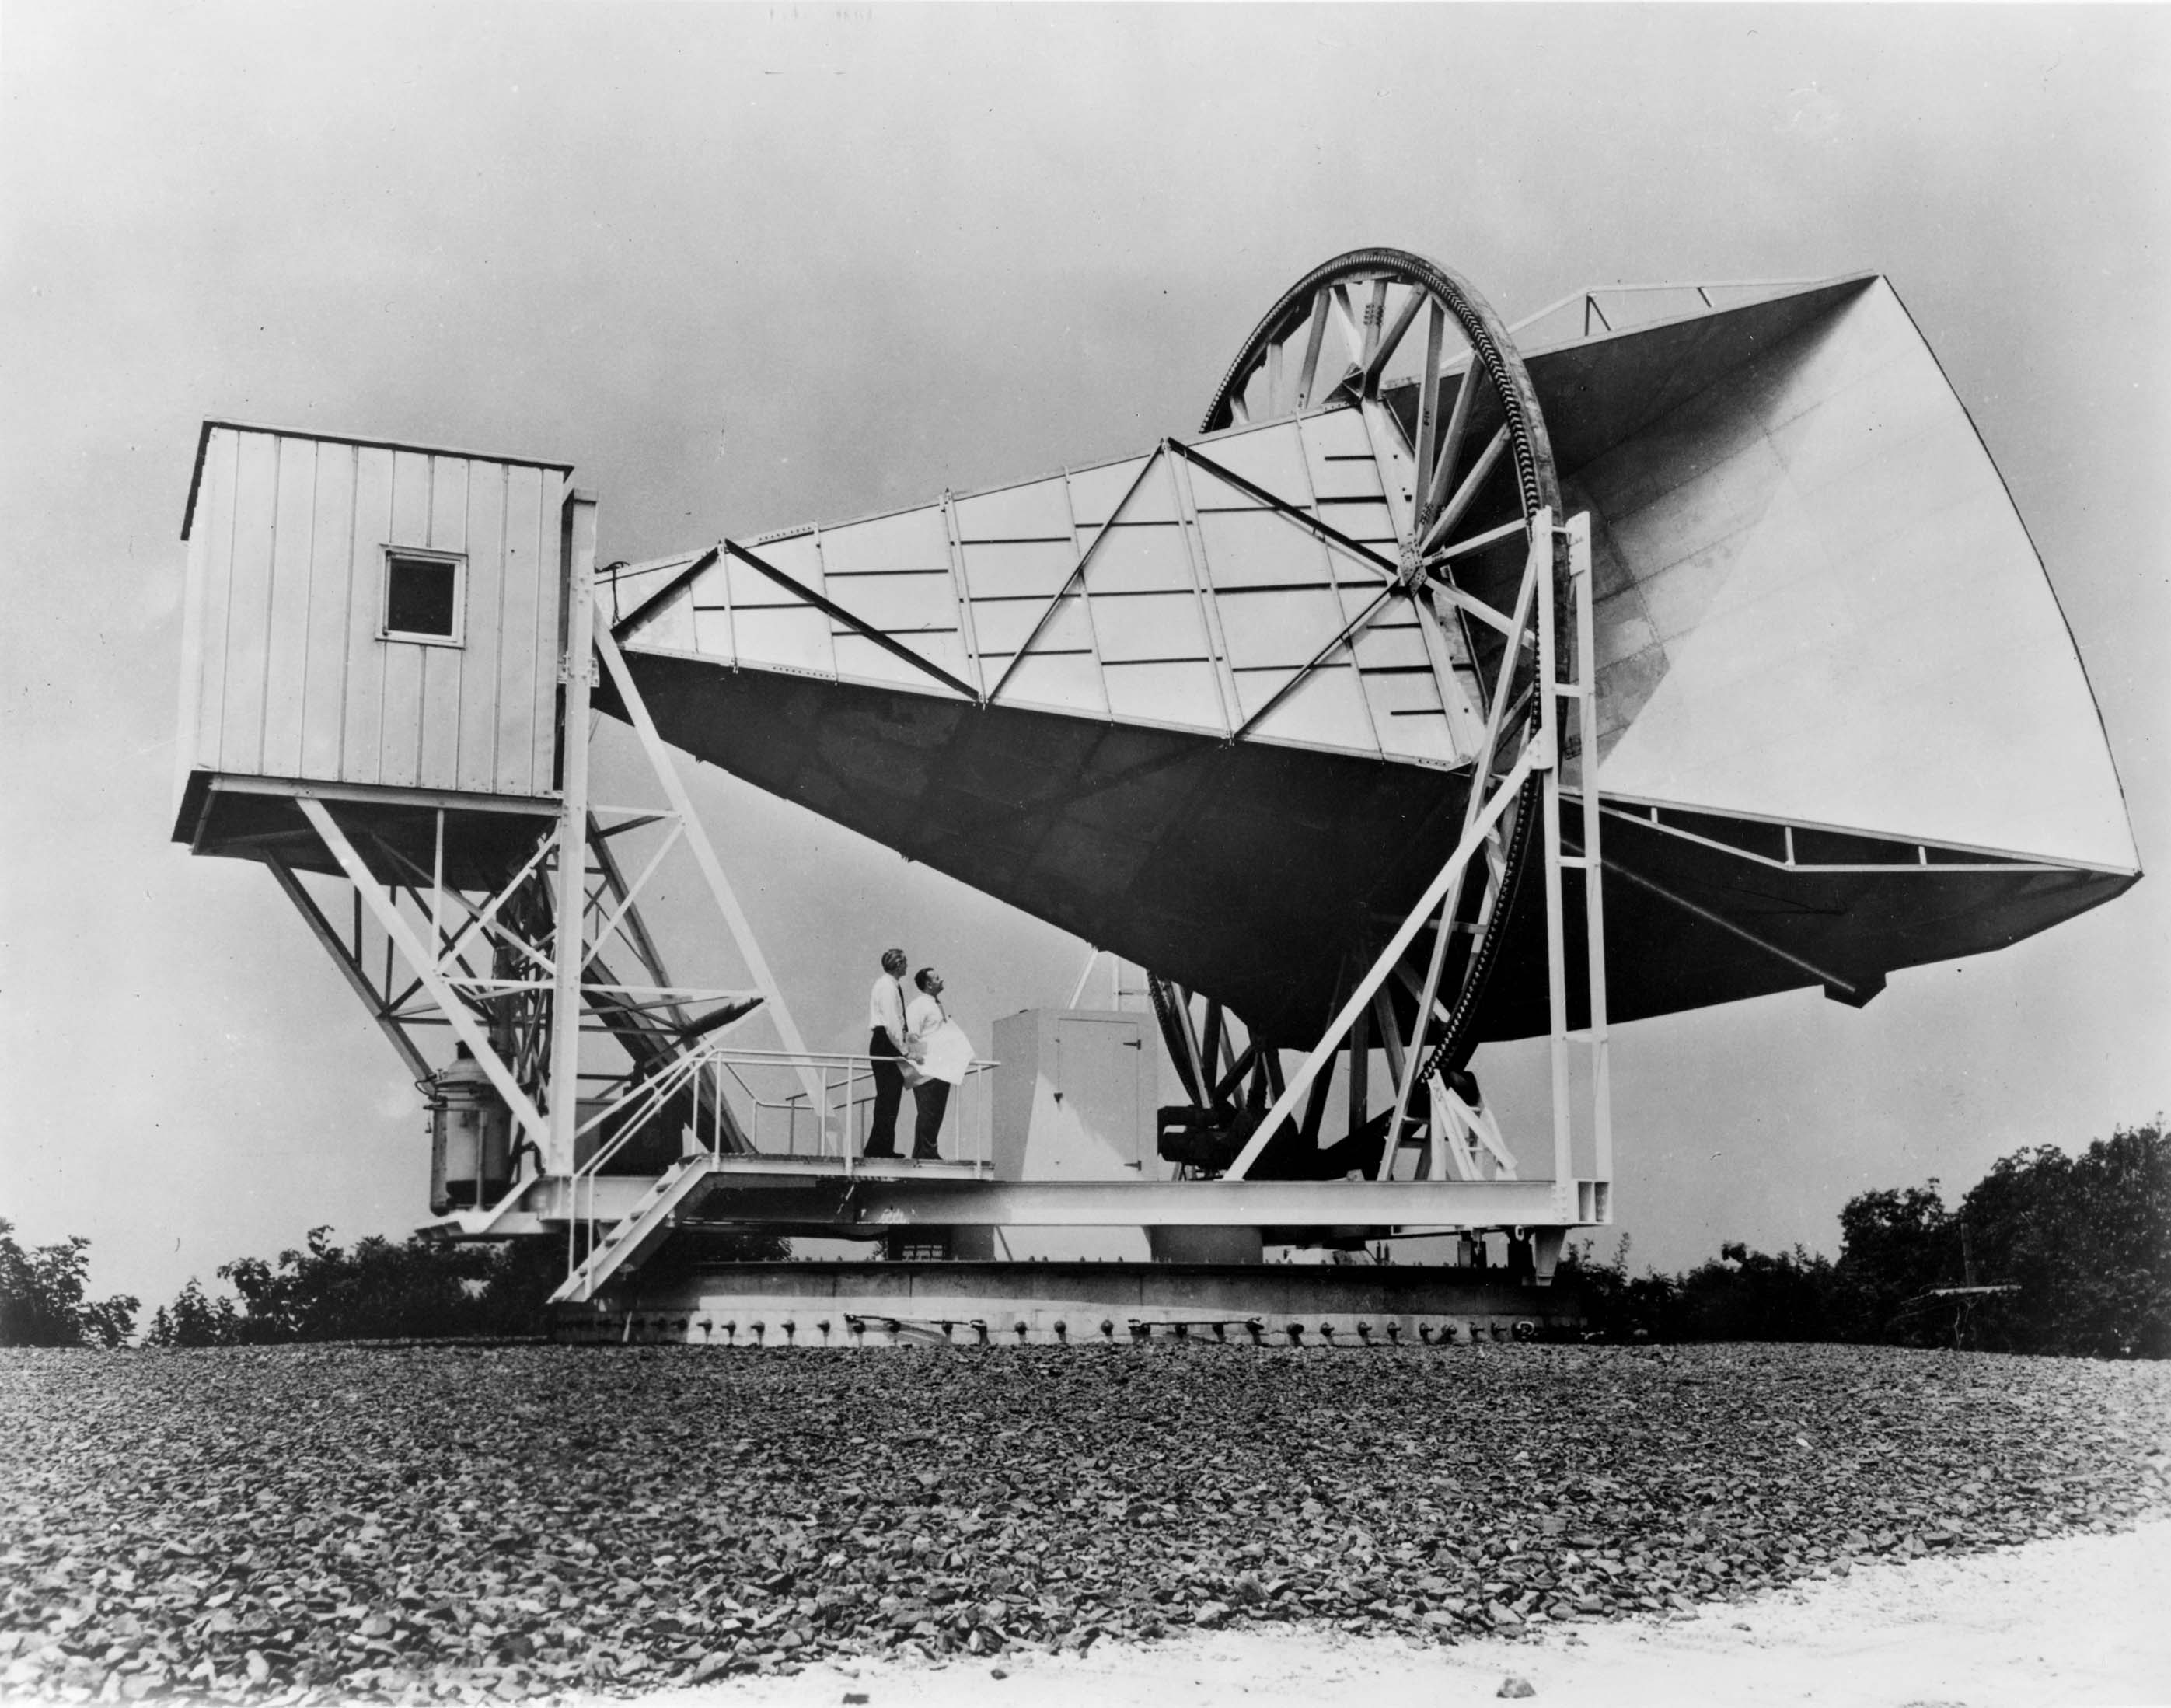
\includegraphics[width=\textwidth]{ch18_cmb_telescope.jpg}
	\end{center}
	\column{.5\textwidth}
	\begin{itemize}
	  \item Such an age would predict a very far distance from us
	  \item Also predicts a high redshift (z=1100)
	  \item If the universe was initially as hot and glowing as a star
		\begin{itemize}
		  \item Such light would be redshifted into microwaves these days
		\end{itemize}
	  \item 1965: Found weird radio signal coming equally from all parts of the universe
		\begin{itemize}
		  \item Like a background noise
		  \item Cleaning or calibrating their telescope couldn't get rid of it
		\end{itemize}
	  \item Now known as the \alert{Cosmic Microwave Background} or CMB
	\end{itemize}
  \end{columns}
\end{frame}

\begin{frame}{The Cosmic Microwave Background}
  \begin{center}
	\begin{tikzpicture}
	  \node<1>[label={below:1965 Image}] at (0,0) {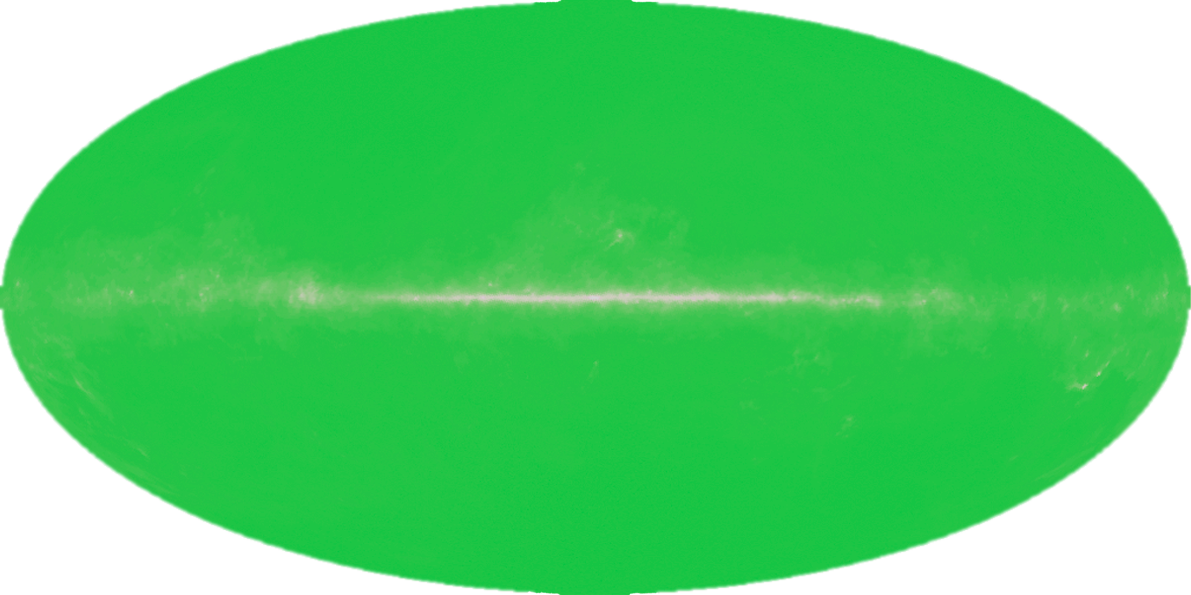
\includegraphics[width=10cm]{ch18_cmb_1965.png}};
	  \node<2>[label={below:Cobe Satellite Image (2006)}] at (0,0) {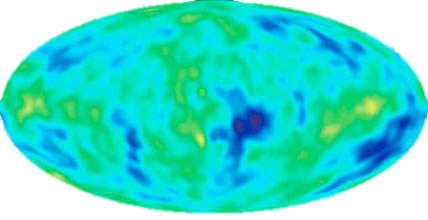
\includegraphics[width=10cm]{ch18_cmb_cobe.png}};
	  \node<3>[label={below:WMAP Satellite Image (2013)}] at (0,0) {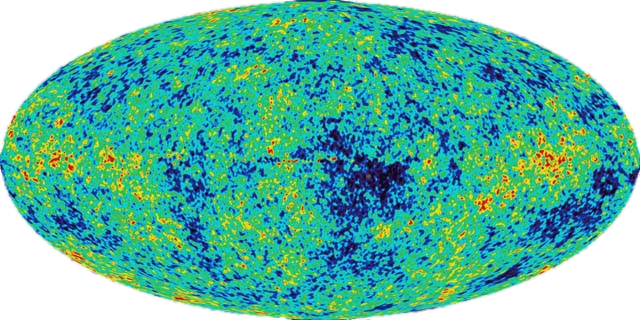
\includegraphics[width=10cm]{ch18_cmb_wmap.png}};
	  \node<4>[label={below:Planck Satellite Image (2016)}] at (0,0) {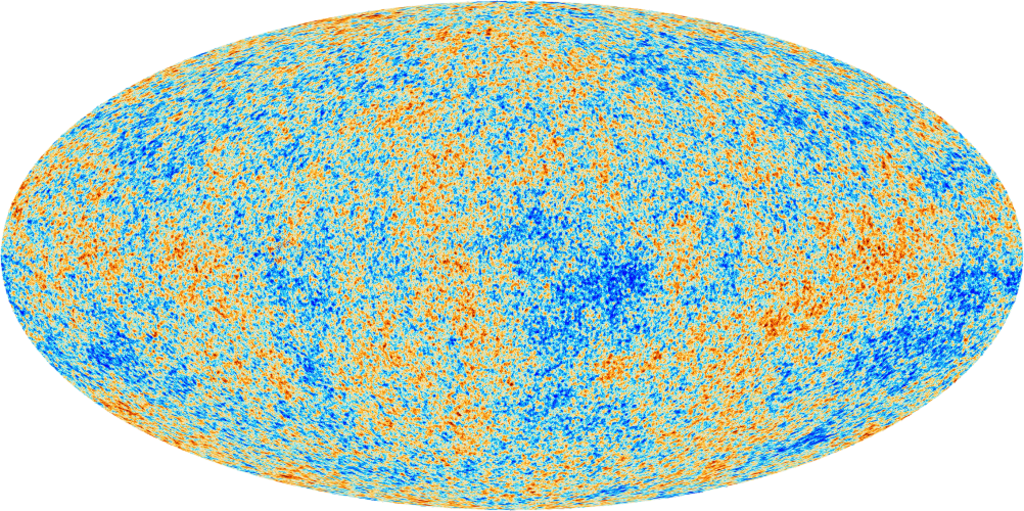
\includegraphics[width=10cm]{ch18_cmb_plank.png}};
	\end{tikzpicture}
  \end{center}
\end{frame}

\begin{frame}{The Most Perfect Blackbody}
  \begin{center}
	\includegraphics[width=.6\textwidth]{ch18_Cmbr.pdf}
  \end{center}
\end{frame}

\begin{frame}{CMB Facts}
  \begin{itemize}
	\item Originally about \SI{3000}{\kelvin} now \SI{2.7260}{\kelvin}
	\item The red and blue patches are hot/cold areas
	  \begin{itemize}
		\item Differ by less than \SI{1e-5}{\kelvin}!
		\item Incredibly smooth
	  \end{itemize}
	\item Furthest back we can look directly
  \end{itemize}
  \begin{center}
	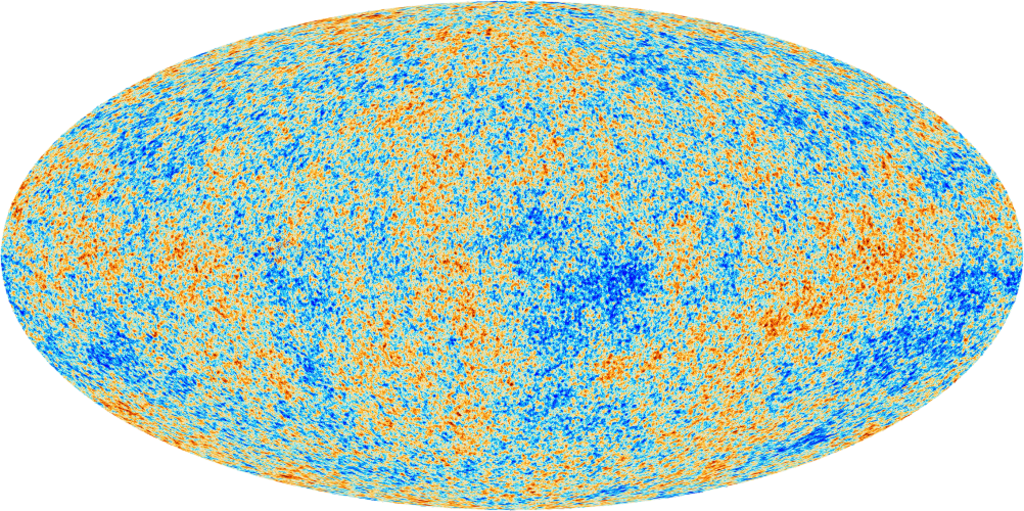
\includegraphics[width=.6\textwidth]{ch18_cmb_plank.png}
  \end{center}
\end{frame}

\begin{frame}{Conclusions}
  \begin{itemize}
	\item Universe was much smoother than it is today
	  \begin{itemize}
		\item We see temperature variations of thousands of kelvin, not $10^{-5}$\ldots
	  \end{itemize}
	\item But still not PERFECTLY smooth
	  \begin{itemize}
		\item Some matter was still clumping before stars and galaxies
	  \end{itemize}
	\item Size scale of patches serves as a valuable tool for model fitting
  \end{itemize}
  \begin{center}
	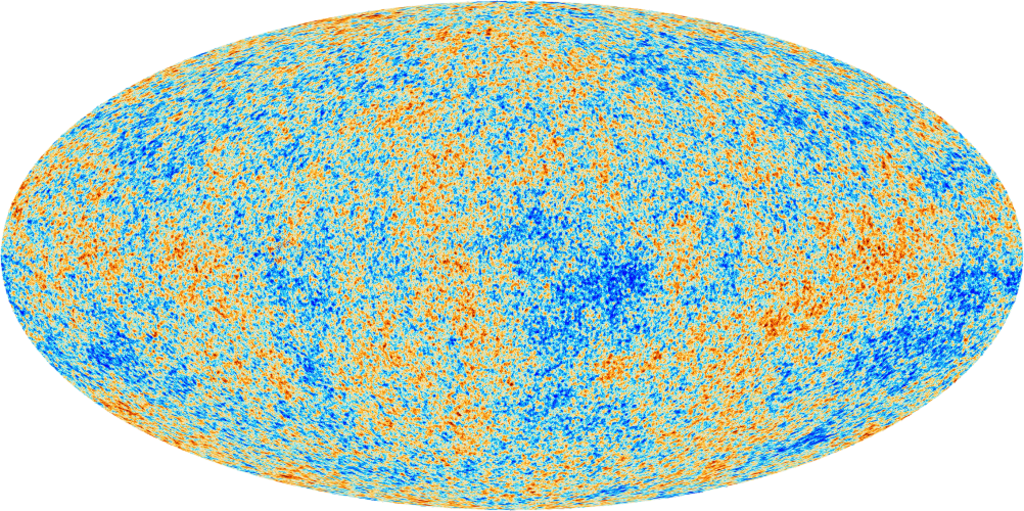
\includegraphics[width=.6\textwidth]{ch18_cmb_plank.png}
  \end{center}
\end{frame}

\begin{frame}{Model Fitting with the CMB}
  \url{http://map.gsfc.nasa.gov/resources/camb_tool}
\end{frame}

\begin{frame}{Other Support for the BBT}
  \begin{itemize}
	\item We see Helium everywhere in the universe
	  \begin{itemize}
		\item Accounts for a solid 25\% of all the mass in the universe
	  \end{itemize}
	\item Helium is spread move evenly across the universe than could be explained by star fusion
	\item Indicates things must have been hot enough in the early universe for large scale fusion to be occuring
	\item Also true of other trace elements like deuterium formed from fusion
	\item How much of the initial matter of the universe ``started'' as different elements influences the abundances we should see today
  \end{itemize}
\end{frame}

\begin{frame}{Understanding Check}
  Suppose the cosmic microwave background had been discovered instead at a much longer wavelength, say large radio waves. This could have implied any of the following \alert{except}:
  \begin{enumerate}
	\item Our universe is older than we thought
	\item Recombination happened earlier in the universe than we thought
	\item \alert<2>{The universe is smoother than we had thought}
	\item The early universe was not as hot as we thought
  \end{enumerate}
\end{frame}

%\fullFrameImage{ch18_planck_history.jpg}

\begin{frame}{Peering past the CMB}
  \begin{itemize}
	\item How could we peer back further than the CMB?
	  \begin{itemize}
		\item Neutrinos
		  \begin{itemize}
			\item Can we observe enough coming from that time to make a reasonable picture?
		  \end{itemize}
		\item Gravity Waves
		  \begin{itemize}
			\item Recently confirmed to have been observed
			\item Fluctuations in space-time, so ```opacity'' doesn't matter
			\item How can we best use them? Still very new (and exciting!)
		  \end{itemize}
	  \end{itemize}
  \end{itemize}
\end{frame}

\begin{frame}{Other CMB Concerns}
  \begin{itemize}
	\item Looking at the CMB, some other questions spring to mind:
	  \begin{itemize}
		\item Why is the universe flat?
		\item Why is the universe so smooth on large scales, but so lumpy on small scales?
	  \end{itemize}
  \end{itemize}
  \begin{center}
	\begin{tikzpicture}[scale=.8, transform shape]
	  \node<1>[label={below:Smooth at large scales}] at (0,0) {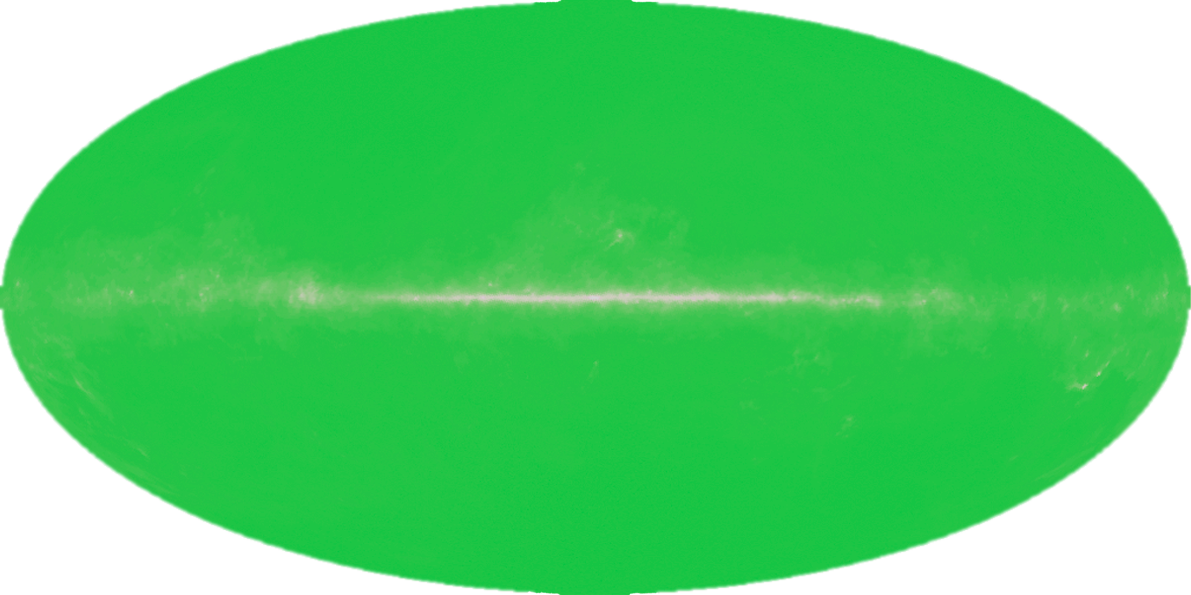
\includegraphics[width=.8\textwidth]{ch18_cmb_1965.png}};
	  \node<2>[label={below:Lumpy at small scales}] at (0,0) {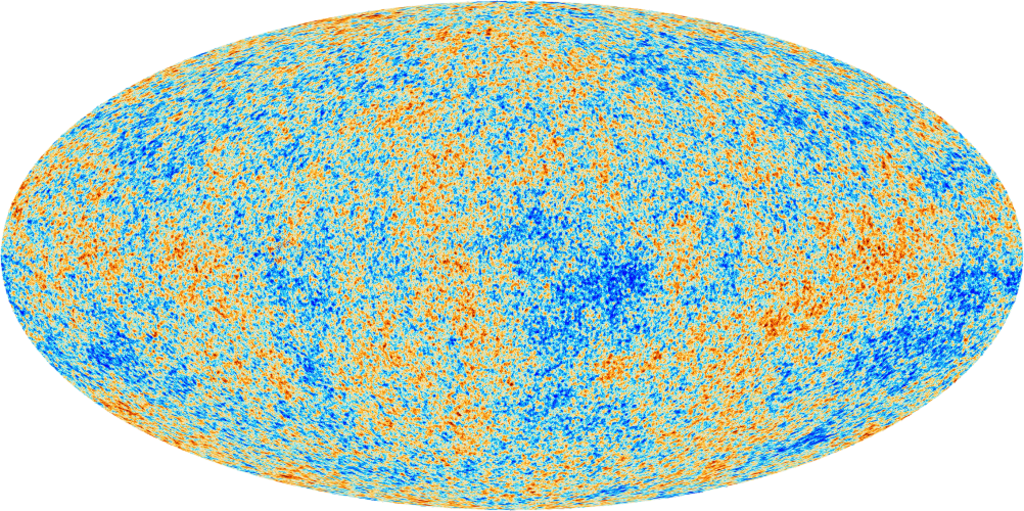
\includegraphics[width=.8\textwidth]{ch18_cmb_plank.png}};
	\end{tikzpicture}
  \end{center}
\end{frame}

\begin{frame}{Houston, We Have a Problem \scriptsize{(Several actually)}}
  \begin{itemize}
	\item Recall that:
	  \begin{center}
		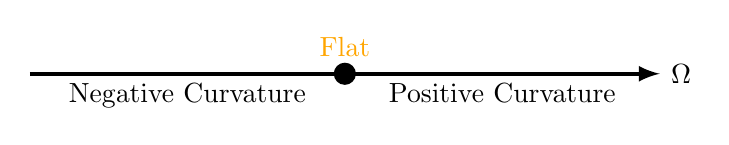
\begin{tikzpicture}
		  \draw[-latex, ultra thick] (-4,0) -- (4,0) node[right] {$\Omega$};
		  \fill (0,0) circle (4pt);
		  \node[below] at (-2,0) {Negative Curvature};
		  \node[below] at (2,0) {Positive Curvature};
		  \node[above, Orange] at (0,.1) {Flat};
		\end{tikzpicture}
	  \end{center}
	\item There are WAY more ways to be curved that flat!
  \end{itemize}
  \begin{columns}[t]
	\column{.5\textwidth}
	\begin{itemize}
	  \item Does something in the underlying physics force flatness? Or how is this so finely tuned?
	  \item Called the Flatness Problem
	\end{itemize}
	\column{.5\textwidth}
	\begin{center}
	  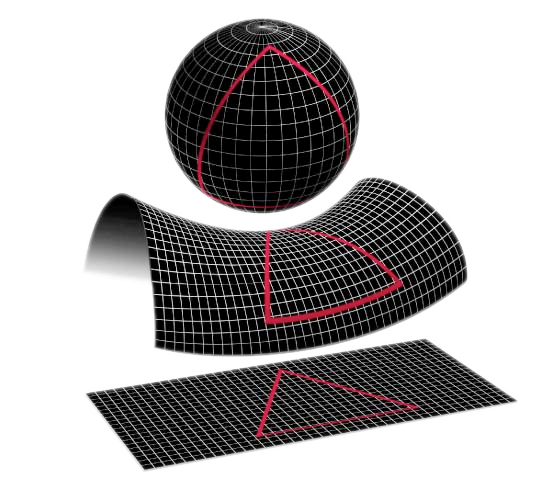
\includegraphics[width=.6\textwidth]{ch18_curvature.png}
	\end{center}
  \end{columns}
\end{frame}

\begin{frame}{The Horizon Problem}
  \begin{itemize}
	\item When we look one direction, we see the CMB 13.3 billion light-years from us
	\item When we look the other direction, we see the same
	\item These two points of the universe can not have ``talked'' to each other!
	  \begin{itemize}
		\item Too far apart for light to travel that far in the age of the universe
	  \end{itemize}
	\item So it is weird that they look so similar
	  \begin{itemize}
		\item We'd expect one to have no influence on the other, so they could look completely different
	  \end{itemize}
	\item Why are they the same?
  \end{itemize}
\end{frame}

\begin{frame}{The Lumpy Problem (Anisotropy)}
  \begin{itemize}
	\item The universe is incredibly smooth on large scales
	\item But decidedly lumpy at small scales
	\item Why this difference?
  \end{itemize}
  \begin{center}
	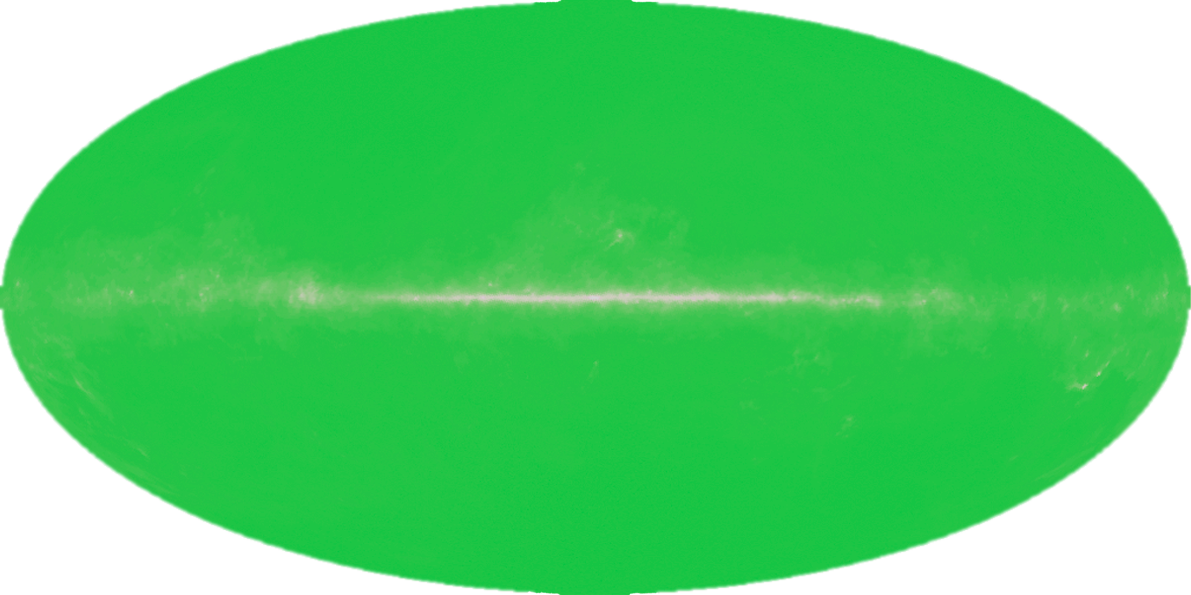
\includegraphics[width=.45\textwidth]{ch18_cmb_1965.png}
	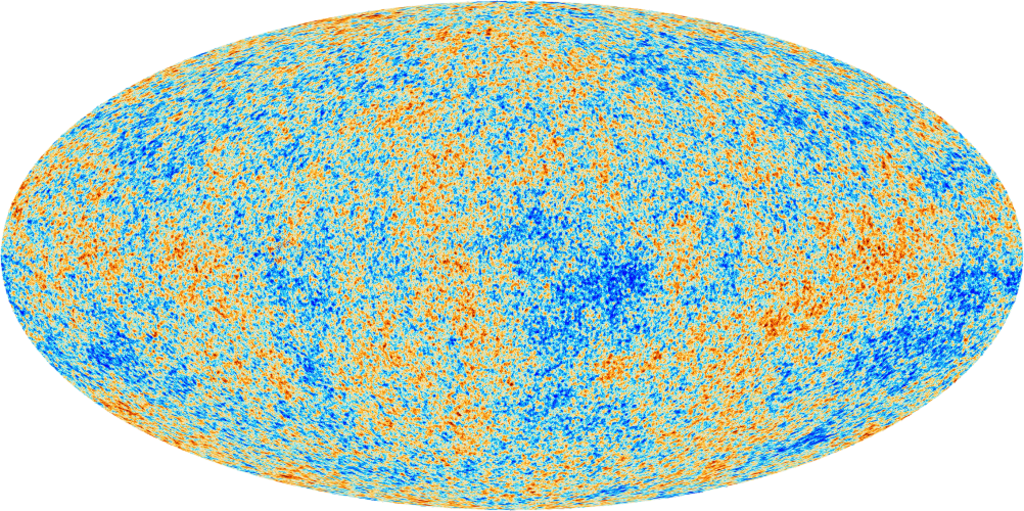
\includegraphics[width=.45\textwidth]{ch18_cmb_plank.png}
  \end{center}
\end{frame}

\begin{frame}{Inflation \scriptsize{(Affecting the universe as well as your bank account\ldots)}}
  \begin{itemize}
	\item Theorized that there must have been a period of EXTREME expansion in the VERY early universe
	\item Grew by some 58 orders of magnitude in maybe $10^{-32}$ seconds\ldots
  \end{itemize}
  \begin{columns}
	\column{.5\textwidth}
	\begin{itemize}
	  \item Solves all three problems
		\begin{itemize}
		  \item Anything looks flat when large enough
		  \item Different parts of the universe could ``talk'' before inflation, equalizing themselves
		\end{itemize}
	\end{itemize}
	\column{.5\textwidth}
	\begin{center}
	  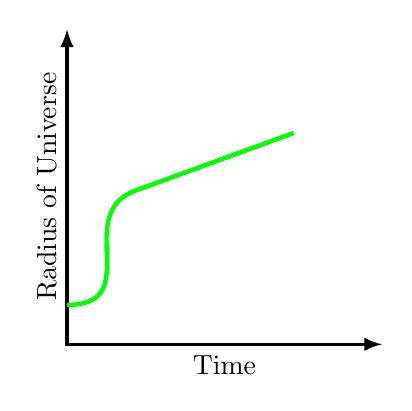
\begin{tikzpicture}
		\draw[latex-latex, very thick] (4,0) -- (0,0) node[midway,below] {Time} -- (0,4) node[midway,above,sloped] {Radius of Universe};
		\draw[green, ultra thick, rounded corners] (0,0.5) ..controls +(0:1) and +(200:1).. (1,2) --+(20:2);
	  \end{tikzpicture}
	\end{center}
  \end{columns}
\end{frame}

\begin{frame}{Quantum Fluctuations}
  \begin{itemize}
	\item Quantum mechanics says that, on the small scale, nothing can be known 100\% certainly
	\item Heisenberg's Uncertainty Principle
	  \[\Delta x \cdot \Delta p \geq \frac{\hbar}{2}\]
	\item The more precisely you know something's position, the less precisely you'll know its velocity!
	\item Results in tiny quantum ripples, of deviance and change
  \end{itemize}
\end{frame}

\begin{frame}{Issues Solved! (Kinda)}
  \begin{itemize}
	\item Inflation takes these tiny ripples and magnifies them to galactic scales
	\item Provide the initial deviations in the universe to start allowing gravity to start the real clumping process
	\item But what causes inflation?
	  \begin{itemize}
		\item Still not well understood
		\item Generally accepted as true at the moment, because it explains most models so well
		\item Perhaps neutrino or gravity wave detectors that could peer past the CMB could shed light ($\leftarrow$ anti-pun?) on the situation
	  \end{itemize}
  \end{itemize}
\end{frame}
%Flatness problem
%Horizon problem
%Lumpiness problem


\end{document}
